% Options for packages loaded elsewhere
\PassOptionsToPackage{unicode}{hyperref}
\PassOptionsToPackage{hyphens}{url}
\PassOptionsToPackage{dvipsnames,svgnames,x11names}{xcolor}
%
\documentclass[
  letterpaper,
  DIV=11,
  numbers=noendperiod]{scrartcl}

\usepackage{amsmath,amssymb}
\usepackage{iftex}
\ifPDFTeX
  \usepackage[T1]{fontenc}
  \usepackage[utf8]{inputenc}
  \usepackage{textcomp} % provide euro and other symbols
\else % if luatex or xetex
  \usepackage{unicode-math}
  \defaultfontfeatures{Scale=MatchLowercase}
  \defaultfontfeatures[\rmfamily]{Ligatures=TeX,Scale=1}
\fi
\usepackage{lmodern}
\ifPDFTeX\else  
    % xetex/luatex font selection
\fi
% Use upquote if available, for straight quotes in verbatim environments
\IfFileExists{upquote.sty}{\usepackage{upquote}}{}
\IfFileExists{microtype.sty}{% use microtype if available
  \usepackage[]{microtype}
  \UseMicrotypeSet[protrusion]{basicmath} % disable protrusion for tt fonts
}{}
\makeatletter
\@ifundefined{KOMAClassName}{% if non-KOMA class
  \IfFileExists{parskip.sty}{%
    \usepackage{parskip}
  }{% else
    \setlength{\parindent}{0pt}
    \setlength{\parskip}{6pt plus 2pt minus 1pt}}
}{% if KOMA class
  \KOMAoptions{parskip=half}}
\makeatother
\usepackage{xcolor}
\usepackage[top=30mm,left=30mm]{geometry}
\setlength{\emergencystretch}{3em} % prevent overfull lines
\setcounter{secnumdepth}{5}
% Make \paragraph and \subparagraph free-standing
\ifx\paragraph\undefined\else
  \let\oldparagraph\paragraph
  \renewcommand{\paragraph}[1]{\oldparagraph{#1}\mbox{}}
\fi
\ifx\subparagraph\undefined\else
  \let\oldsubparagraph\subparagraph
  \renewcommand{\subparagraph}[1]{\oldsubparagraph{#1}\mbox{}}
\fi


\providecommand{\tightlist}{%
  \setlength{\itemsep}{0pt}\setlength{\parskip}{0pt}}\usepackage{longtable,booktabs,array}
\usepackage{calc} % for calculating minipage widths
% Correct order of tables after \paragraph or \subparagraph
\usepackage{etoolbox}
\makeatletter
\patchcmd\longtable{\par}{\if@noskipsec\mbox{}\fi\par}{}{}
\makeatother
% Allow footnotes in longtable head/foot
\IfFileExists{footnotehyper.sty}{\usepackage{footnotehyper}}{\usepackage{footnote}}
\makesavenoteenv{longtable}
\usepackage{graphicx}
\makeatletter
\def\maxwidth{\ifdim\Gin@nat@width>\linewidth\linewidth\else\Gin@nat@width\fi}
\def\maxheight{\ifdim\Gin@nat@height>\textheight\textheight\else\Gin@nat@height\fi}
\makeatother
% Scale images if necessary, so that they will not overflow the page
% margins by default, and it is still possible to overwrite the defaults
% using explicit options in \includegraphics[width, height, ...]{}
\setkeys{Gin}{width=\maxwidth,height=\maxheight,keepaspectratio}
% Set default figure placement to htbp
\makeatletter
\def\fps@figure{htbp}
\makeatother

\KOMAoption{captions}{tableheading}
\makeatletter
\makeatother
\makeatletter
\makeatother
\makeatletter
\@ifpackageloaded{caption}{}{\usepackage{caption}}
\AtBeginDocument{%
\ifdefined\contentsname
  \renewcommand*\contentsname{Table of contents}
\else
  \newcommand\contentsname{Table of contents}
\fi
\ifdefined\listfigurename
  \renewcommand*\listfigurename{List of Figures}
\else
  \newcommand\listfigurename{List of Figures}
\fi
\ifdefined\listtablename
  \renewcommand*\listtablename{List of Tables}
\else
  \newcommand\listtablename{List of Tables}
\fi
\ifdefined\figurename
  \renewcommand*\figurename{Figure}
\else
  \newcommand\figurename{Figure}
\fi
\ifdefined\tablename
  \renewcommand*\tablename{Table}
\else
  \newcommand\tablename{Table}
\fi
}
\@ifpackageloaded{float}{}{\usepackage{float}}
\floatstyle{ruled}
\@ifundefined{c@chapter}{\newfloat{codelisting}{h}{lop}}{\newfloat{codelisting}{h}{lop}[chapter]}
\floatname{codelisting}{Listing}
\newcommand*\listoflistings{\listof{codelisting}{List of Listings}}
\makeatother
\makeatletter
\@ifpackageloaded{caption}{}{\usepackage{caption}}
\@ifpackageloaded{subcaption}{}{\usepackage{subcaption}}
\makeatother
\makeatletter
\makeatother
\ifLuaTeX
  \usepackage{selnolig}  % disable illegal ligatures
\fi
\IfFileExists{bookmark.sty}{\usepackage{bookmark}}{\usepackage{hyperref}}
\IfFileExists{xurl.sty}{\usepackage{xurl}}{} % add URL line breaks if available
\urlstyle{same} % disable monospaced font for URLs
\hypersetup{
  pdftitle={EJERCICIOS C1T2},
  pdfauthor={Betancourt Alison; Angulo Javier; Anrango Stalin; Huilca Fernando; Sarasti Sebastian; Simbaña Mateo},
  colorlinks=true,
  linkcolor={blue},
  filecolor={Maroon},
  citecolor={Blue},
  urlcolor={Blue},
  pdfcreator={LaTeX via pandoc}}

\title{EJERCICIOS C1T2}
\author{Betancourt Alison \and Angulo Javier \and Anrango
Stalin \and Huilca Fernando \and Sarasti Sebastian \and Simbaña Mateo}
\date{}

\begin{document}
\maketitle
\renewcommand*\contentsname{Contenido}
{
\hypersetup{linkcolor=}
\setcounter{tocdepth}{3}
\tableofcontents
}
\hypertarget{ejercicios---el-lenguaje-de-las-matematicas}{%
\section{Ejercicios - El lenguaje de las
matematicas}\label{ejercicios---el-lenguaje-de-las-matematicas}}

\begin{enumerate}
\def\labelenumi{\arabic{enumi}.}
\setcounter{enumi}{26}
\tightlist
\item
  Un grupo de 191 estudiantes, de los cuales 10 toman francés, negocios
  y música; 36 toman francés y negocios; 20 están en francés y música;
  18 en negocios y música; 65 en francés; 76 en negocios y 63 toman
  música
\end{enumerate}

\hypertarget{respuesta}{%
\section{Respuesta:}\label{respuesta}}

∣A∪B∣=∣A∣+∣B∣−∣A∩B∣

\textbf{19 + 10 + 10 + 26 + 8 + 32 = 105}

\hypertarget{ejercicio-7}{%
\section{EJERCICIO 7}\label{ejercicio-7}}

\textbf{En los ejercicios 1 al 16, establezca el universo como el
conjunto} \(U=\{1, 2, 3, . . . , 10\}\). Sea \(A=\{1, 4, 7, 10\}\),
\(B=\{1, 2, 3, 4, 5\}\) y \(C=\{2,4, 6, 8\}\)\textbf{. Liste los
elementos de cada conjunto:}

\(U' = \emptyset\) ,el complemento del conjunto universo es el conjunto
vacio.

\hypertarget{ejercicio-22}{%
\section{EJERCICIO 22}\label{ejercicio-22}}

\textbf{En los ejercicios 17 al 24, dibuje un diagrama de Venn y sombree
el conjunto indicado.}

Dado que el universo es \(U=\{1, 2, 3, . . . , 10\}\), y los conjuntos
son:

\(A = \{1,4,7,10\}\)

\(B = \{1,2,3,4,5\}\)

\(C = \{2,4,6,8\}\)

Calculamos los complementos de A y C:

\(A^{c} = \{2, 3, 5, 6, 8 ,9\}\)

\(C^{c} = \{1, 3, 5, 7, 9, 10\}\)

Luego, calculamos las operaciones de unión:

\((A^{c} ∪ B) = \{1,2,3,4,5,6,8,9\}\)

\((C^{c} - A) = \{3,5,9\}\)

Finalmente, calculamos la intersección de los dos conjuntos anteriores:

\((A^{c} ∪ B) ∩ (C^{c} - A) = \{3,5,9\}\)

El diagrama de Venn correspondiente se muestra a continuación:

\begin{figure}

{\centering 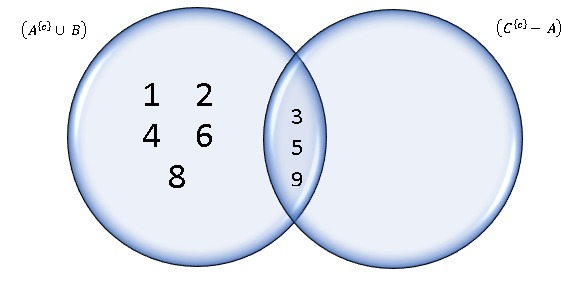
\includegraphics{venn.jpg}

}

\caption{Diagrama de Venn}

\end{figure}

\hypertarget{ejercicio-27}{%
\section{EJERCICIO 27}\label{ejercicio-27}}

Un grupo de 191 estudiantes, de los cuales 10 toman francés, negocios y
música; 36 toman francés y negocios; 20 están en francés y música; 18 en
negocios y música; 65 en francés; 76 en negocios y 63 toman música

\textbf{Respuesta:} ∣A∪B∣=∣A∣+∣B∣−∣A∩B∣

\textbf{19 + 10 + 10 + 26 + 8 + 32 = 105}

\hypertarget{ejercicio-51}{%
\section{EJERCICIO 51}\label{ejercicio-51}}

\textbf{En los ejercicios 48 al 52, determine si cada par de conjuntos
es igual} \(A=\{x|x^2+x=2\}\),\(B=\{1,-2\}\)

\[
\begin{align*}
x^2 + x &= 2 \\
x^2 + x - 2 &= 0 \\
(x + 2)(x - 1) &= 0 \\
x_1 = -2 \quad& x_2 = 1\\
\end{align*}
\]

\(\therefore A=\{1,-2\}\)=\(B=\{1,-2\}\) \textbf{Por lo tanto el par de
conjuntos son iguales}

\hypertarget{ejercicio-52}{%
\section{EJERCICIO 52}\label{ejercicio-52}}

\textbf{Determine si cada par de conjuntos es igual:}

\(\{x│ x\ es\ un\ número\ real\ y\ 0 < x \leq 2\}\), \(\{1,2\}\).

Hay que tomar en cuenta, que dos conjuntos son iguales si tienen los
mismos elementos.

\(A = \{x│ x\ es\ un\ número\ real\ y\ 0 < x \leq 2\}\). En el conjunto
\textbf{A} podemos denotar que \textbf{x} puede tomar valores mayores a
\emph{0} y menores o igual que \emph{2}, por lo tanto podrían ser
``0.5'', ``1'', ``1.5'', etc.

\(B = \{1,2\}\). En el conjunto \textbf{B} podemos observar que contiene
solamente al 1 y al 2 como elementos del mismo.

\textbf{\emph{RESPUESTA:}} Podemos concluir que el conjunto
\(A = \{x│ x\ es\ un\ número\ real\ y\ 0 < x \leq 2\}\) y el conjunto
\(B = \{1,2\}\), \textbf{NO} son iguales porque \emph{no tienen los
mismos elementos}.

\hypertarget{ejercicio-53}{%
\section{EJERCICIO 53}\label{ejercicio-53}}

Liste los miembros de \(P(\{a, b\})\). ¿Cuáles son los subconjuntos
propios de \(\{a, b\}\)?

Los miembros de \(P(\{a, b\})\) son: \(\emptyset\), \(\{a\}\),
\(\{b\}\), \(\{a,b\}\).

Todos menos \(\{a,b\}\) son subconjuntos propios de \(\{a,b\}\).



\end{document}
